\documentclass[12pt]{article}

\usepackage[spanish]{babel}
\usepackage{amsmath}
\usepackage{amsfonts}
\usepackage[utf8]{inputenx}
\usepackage{algorithm2e}
\usepackage{listings}
\usepackage{pdfpages}

\usepackage{color}
\definecolor{deepblue}{RGB}{0,0,153}
\definecolor{deepred}{RGB}{153,0,0}
\definecolor{deepgreen}{RGB}{51,102,0}
\definecolor{deepyellow}{RGB}{204,204,0}

\lstset{ %
			language=Python,
			basicstyle=\footnotesize,
			numbers=left,
			stepnumber=1,
			numbersep=4pt,
			tabsize=2,
			otherkeywords={self}, 
			keywordstyle=\color{deepred},
			stringstyle=\color{deepgreen},
			commentstyle=\color{deepblue},
}
\usepackage{hyperref}
\hypersetup{
    colorlinks=true,
    citecolor=black,
    filecolor=black,
    linkcolor=black,
    urlcolor=black,
    linktoc=all
}


\title{Distancia de Edición}
\author{
        Alejandro Pernin 
}
\date{\today}



\begin{document}
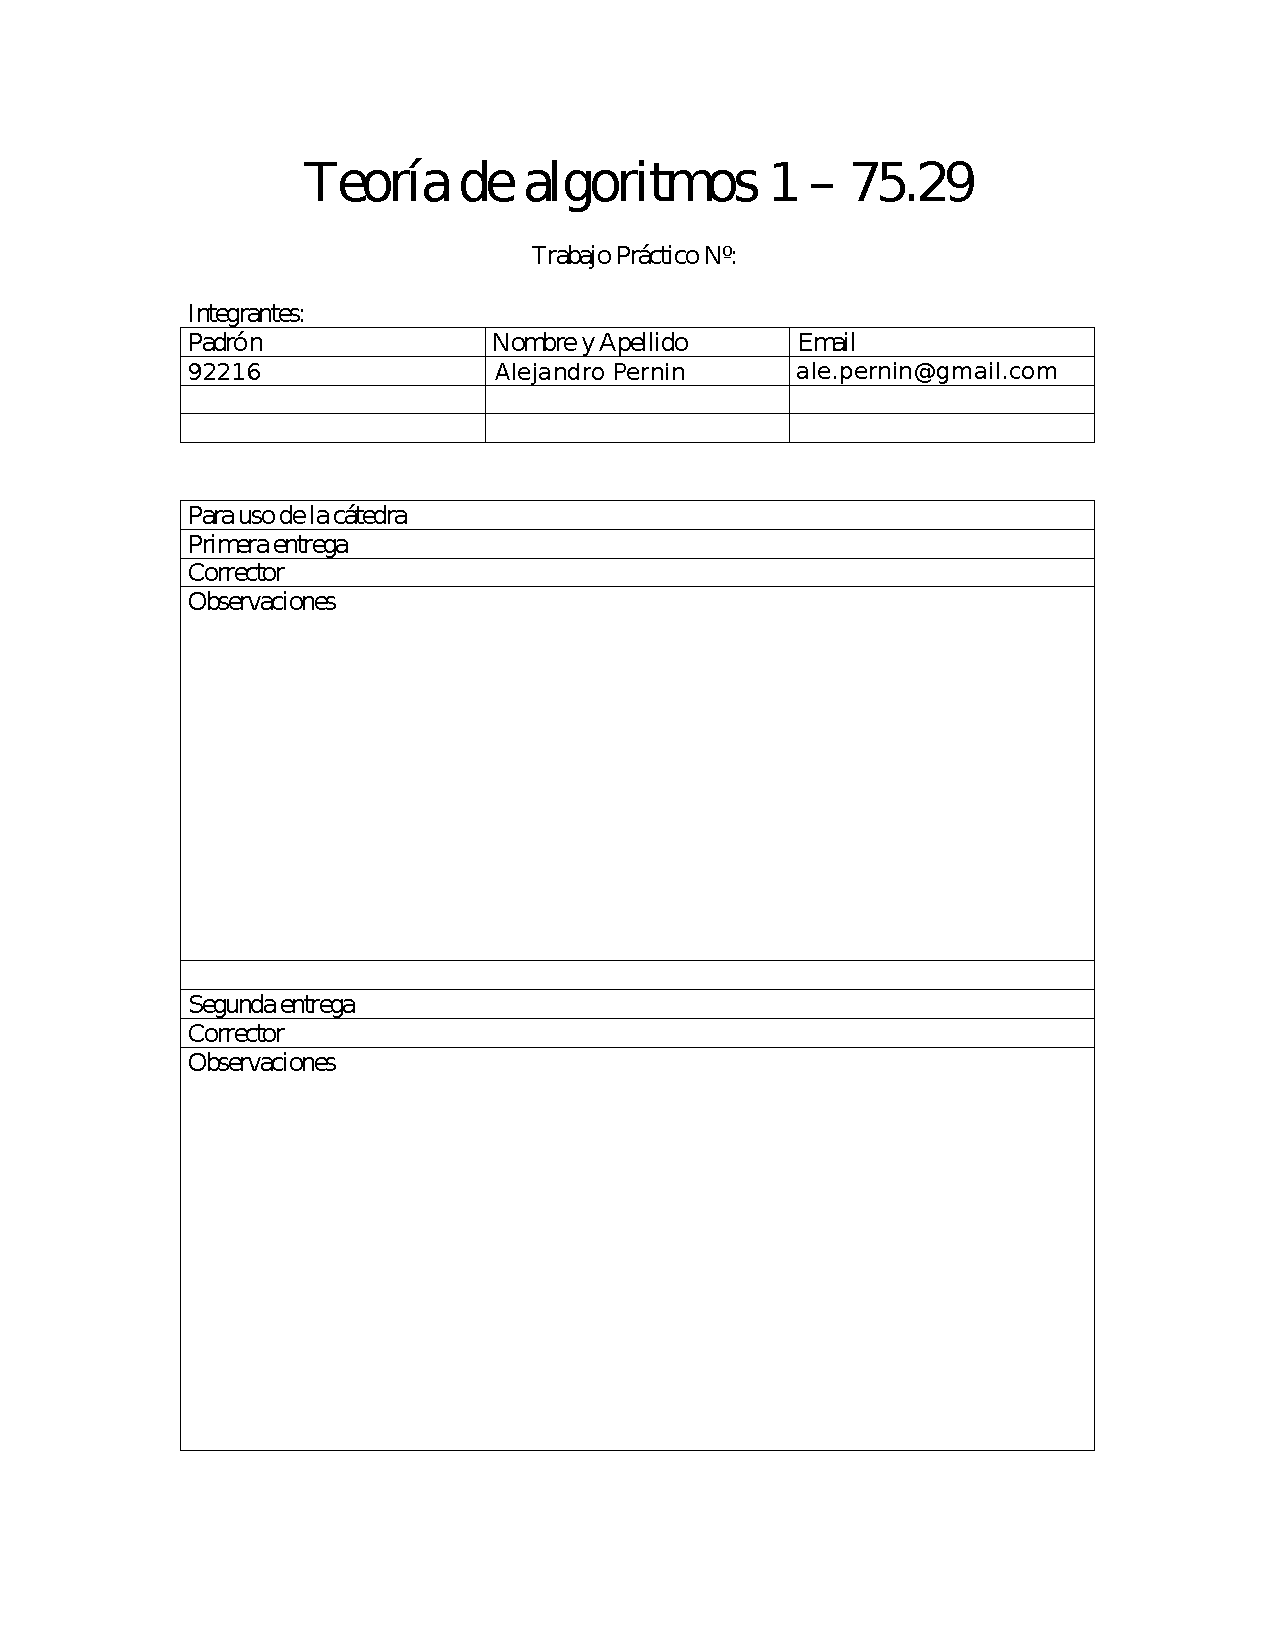
\includepdf{caratulatp.pdf}

\maketitle

\newpage
\tableofcontents

\newpage

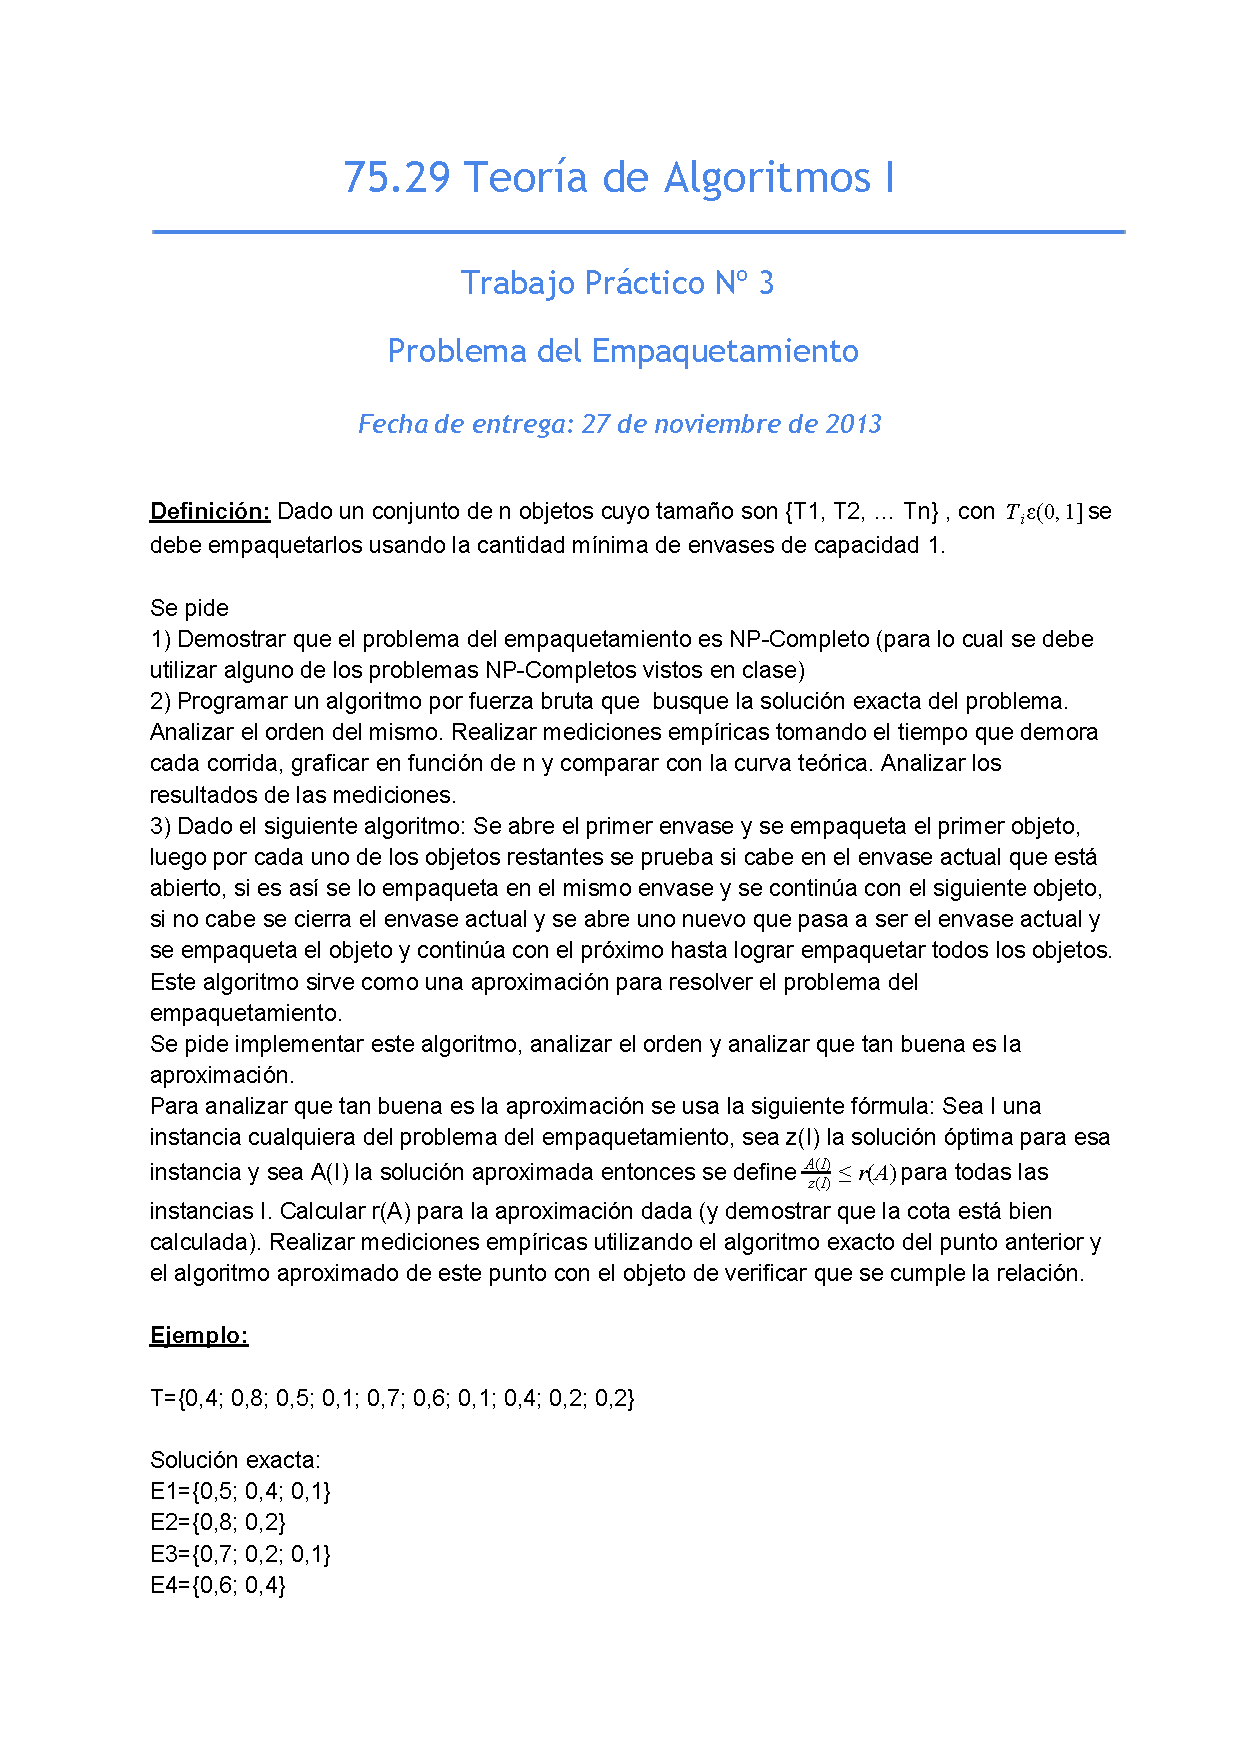
\includepdf[pages=-]{TDATP32013.pdf}

\newpage
\section{Resolucion}
	\subsection{Demostración NP-Completo}
		Para la demostración de que este problema es NP-Completo, se 
		utiliza otro problema cuya demostración de NP-Completo se considera
		ya conocida; reduciendo dicho conocido problema al problema de
		Bin Packing, demostramos que el problema también es NP.
		
		Como problema de referencia se utilizar\'a \emph{Subset Sum}\footnote{\url{http://en.wikipedia.org/wiki/Subset_sum_problem}}.
		Primero definamos ambos problemas:
		\begin{itemize}
			\item \underline{Bin Packing}: $\{ <S,j> | S = \{ s_{1},s_{2}...,s_{n}\}; 0<s_{i}<1,$ 
			y todos los objetos $1,...,n$ deben empaquetarse en envases de capacidad $j$.
			
			\item \underline{Subset Sum}: $\{ <C,k> | C = \{ c_{1},c_{2}...,c_{n}\}$ donde $c_{i}$
			es un entero positivo, y existe algun subconjunto $C'\subseteq C$ tal que la suma de sus
			elementos sume exactamente $k$.
		\end{itemize}
		
		Se considera demostrado y sabido que \emph{Subset Sum} es NP-Completo, 
		por medio de reducción demostraremos que \emph{Bin Packing} también lo es.
		Primero consideramos que \emph{Subset Sum} es NP-Completo aún en un caso restringido:
			\\ 
			
			$k=\sum_{c_{i}\in C}^{n} c_{i}/2 = W/2$
			
		Llamamos a esta instancia \emph{Subset Half Sum}, instancia que
		se demostrara se soluciona facilmente con \emph{Bin Packing}
\end{document}
